\documentclass{standalone}
\usepackage{tikz}
\usetikzlibrary{patterns, positioning}
\usepackage[sfdefault]{ClearSans} %% option 'sfdefault' activates Clear Sans as the default text font
\usepackage[T1]{fontenc}

\begin{document}
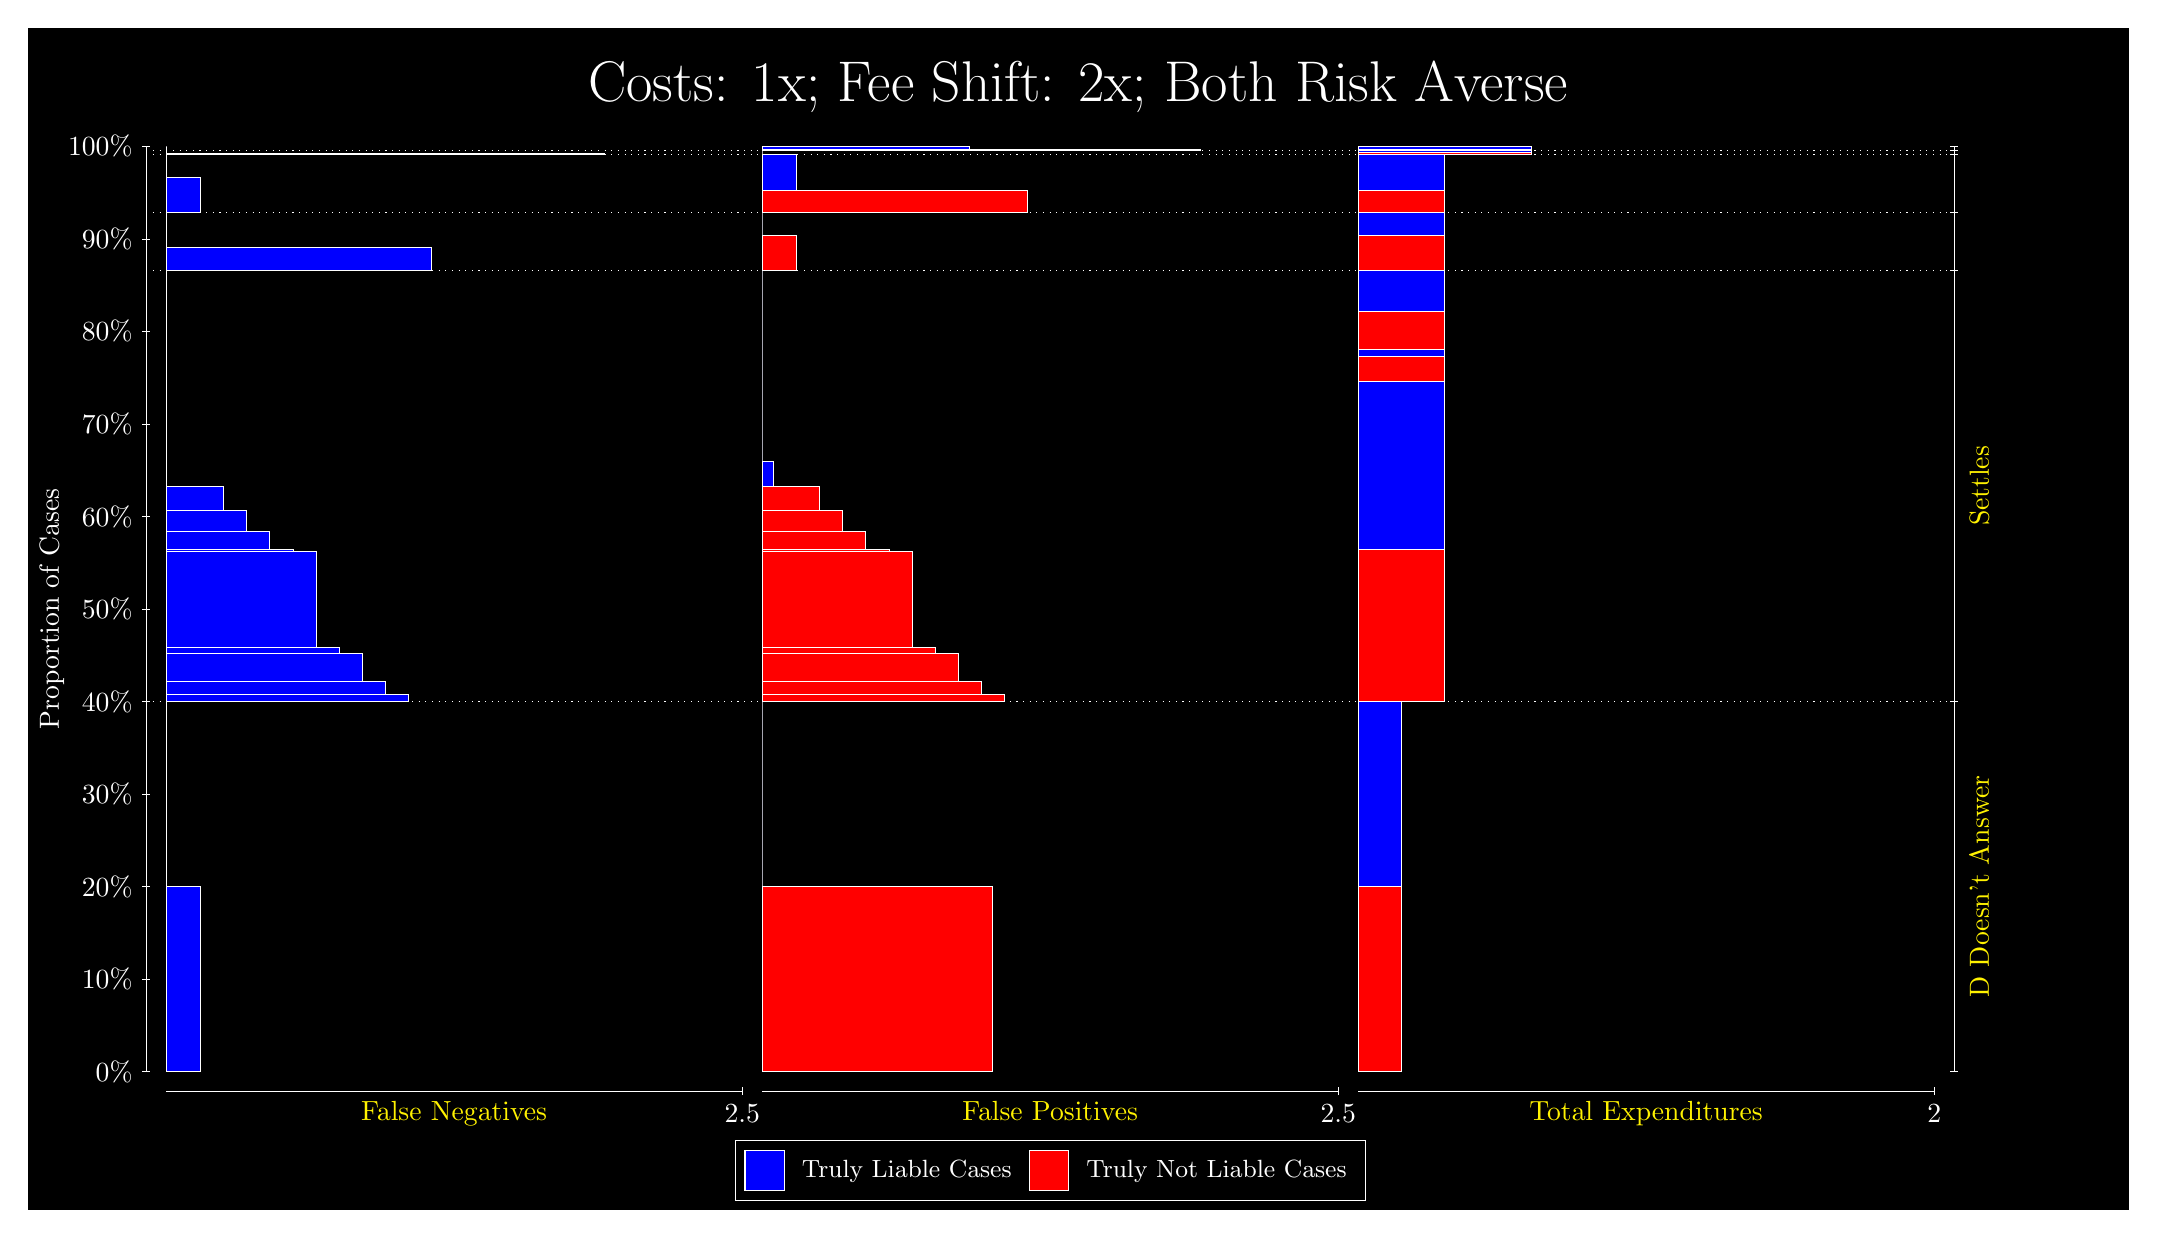
\begin{tikzpicture}
\draw[fill=black] (0,0) rectangle (26.667,15);
\draw[text=white] (0,13.5) rectangle (26.667,15) node[midway] {\huge Costs: 1x; Fee Shift: 2x; Both Risk Averse};
\draw[white, very thin] (1.5,1.75) -- (1.5,13.5);
\node[rotate=90, text=white, anchor=center] at (0.3, 7.625) {Proportion of Cases};
\draw[white, very thin] (1.45,1.75) -- (1.55,1.75);
\node[text=white, anchor=east] at (1.45, 1.75) {0\%};
\draw[white, very thin] (1.45,2.925) -- (1.55,2.925);
\node[text=white, anchor=east] at (1.45, 2.925) {10\%};
\draw[white, very thin] (1.45,4.1) -- (1.55,4.1);
\node[text=white, anchor=east] at (1.45, 4.1) {20\%};
\draw[white, very thin] (1.45,5.275) -- (1.55,5.275);
\node[text=white, anchor=east] at (1.45, 5.275) {30\%};
\draw[white, very thin] (1.45,6.45) -- (1.55,6.45);
\node[text=white, anchor=east] at (1.45, 6.45) {40\%};
\draw[white, very thin] (1.45,7.625) -- (1.55,7.625);
\node[text=white, anchor=east] at (1.45, 7.625) {50\%};
\draw[white, very thin] (1.45,8.8) -- (1.55,8.8);
\node[text=white, anchor=east] at (1.45, 8.8) {60\%};
\draw[white, very thin] (1.45,9.975) -- (1.55,9.975);
\node[text=white, anchor=east] at (1.45, 9.975) {70\%};
\draw[white, very thin] (1.45,11.15) -- (1.55,11.15);
\node[text=white, anchor=east] at (1.45, 11.15) {80\%};
\draw[white, very thin] (1.45,12.325) -- (1.55,12.325);
\node[text=white, anchor=east] at (1.45, 12.325) {90\%};
\draw[white, very thin] (1.45,13.5) -- (1.55,13.5);
\node[text=white, anchor=east] at (1.45, 13.5) {100\%};

\draw[white, very thin] (24.457,1.75) -- (24.457,13.5);
\draw[white, very thin] (24.407,1.75) -- (24.507,1.75);
\node[anchor=west] at (24.407, 1.75) {};
\draw[white, very thin] (24.407,6.45) -- (24.507,6.45);
\node[anchor=west] at (24.407, 6.45) {};
\draw[white, very thin] (24.407,11.926) -- (24.507,11.926);
\node[anchor=west] at (24.407, 11.926) {};
\draw[white, very thin] (24.407,12.66) -- (24.507,12.66);
\node[anchor=west] at (24.407, 12.66) {};
\draw[white, very thin] (24.407,13.393) -- (24.507,13.393);
\node[anchor=west] at (24.407, 13.393) {};
\draw[white, very thin] (24.407,13.447) -- (24.507,13.447);
\node[anchor=west] at (24.407, 13.447) {};
\draw[white, very thin] (24.407,13.5) -- (24.507,13.5);
\node[anchor=west] at (24.407, 13.5) {};

\draw[white, very thin, fill=blue] (1.75,1.75) rectangle (2.1891,4.1);
\draw[white, very thin, fill=red] (1.75,4.1) rectangle (1.75,6.45);
\draw[white, very thin, fill=blue] (1.75,6.45) rectangle (4.8239,6.5362);
\draw[white, very thin, fill=blue] (1.75,6.5362) rectangle (4.5312,6.7108);
\draw[white, very thin, fill=blue] (1.75,6.7108) rectangle (4.2384,7.0592);
\draw[white, very thin, fill=blue] (1.75,7.0592) rectangle (3.9457,7.1402);
\draw[white, very thin, fill=blue] (1.75,7.1402) rectangle (3.6529,8.3605);
\draw[white, very thin, fill=blue] (1.75,8.3605) rectangle (3.3602,8.3874);
\draw[white, very thin, fill=blue] (1.75,8.3874) rectangle (3.0674,8.6102);
\draw[white, very thin, fill=blue] (1.75,8.6102) rectangle (2.7746,8.8733);
\draw[white, very thin, fill=blue] (1.75,8.8733) rectangle (2.4819,9.1879);
\draw[white, very thin, fill=red] (1.75,9.1879) rectangle (1.75,11.926);
\draw[white, very thin, fill=blue] (1.75,11.926) rectangle (5.1167,12.214);
\draw[white, very thin, fill=red] (1.75,12.214) rectangle (1.75,12.66);
\draw[white, very thin, fill=blue] (1.75,12.66) rectangle (2.1891,13.105);
\draw[white, very thin, fill=red] (1.75,13.105) rectangle (1.75,13.393);
\draw[white, very thin, fill=blue] (1.75,13.393) rectangle (7.3123,13.413);
\draw[white, very thin, fill=red] (1.75,13.413) rectangle (1.75,13.447);
\draw[white, very thin, fill=red] (1.75,13.447) rectangle (1.75,13.467);
\draw[white, very thin, fill=blue] (1.75,13.467) rectangle (1.75,13.5);
\draw[white, very thin, fill=red] (9.3189,1.75) rectangle (12.246,4.1);
\draw[white, very thin, fill=blue] (9.3189,4.1) rectangle (9.3189,6.45);
\draw[white, very thin, fill=red] (9.3189,6.45) rectangle (12.393,6.5362);
\draw[white, very thin, fill=red] (9.3189,6.5362) rectangle (12.1,6.7108);
\draw[white, very thin, fill=red] (9.3189,6.7108) rectangle (11.807,7.0592);
\draw[white, very thin, fill=red] (9.3189,7.0592) rectangle (11.515,7.1401);
\draw[white, very thin, fill=red] (9.3189,7.1401) rectangle (11.222,8.3605);
\draw[white, very thin, fill=red] (9.3189,8.3605) rectangle (10.929,8.3874);
\draw[white, very thin, fill=red] (9.3189,8.3874) rectangle (10.636,8.6101);
\draw[white, very thin, fill=red] (9.3189,8.6101) rectangle (10.344,8.8733);
\draw[white, very thin, fill=red] (9.3189,8.8733) rectangle (10.051,9.1879);
\draw[white, very thin, fill=blue] (9.3189,9.1879) rectangle (9.4652,9.5025);
\draw[white, very thin, fill=blue] (9.3189,9.5025) rectangle (9.3189,11.926);
\draw[white, very thin, fill=red] (9.3189,11.926) rectangle (9.758,12.371);
\draw[white, very thin, fill=blue] (9.3189,12.371) rectangle (9.3189,12.66);
\draw[white, very thin, fill=red] (9.3189,12.66) rectangle (12.686,12.948);
\draw[white, very thin, fill=blue] (9.3189,12.948) rectangle (9.758,13.393);
\draw[white, very thin, fill=red] (9.3189,13.393) rectangle (9.3189,13.427);
\draw[white, very thin, fill=blue] (9.3189,13.427) rectangle (9.3189,13.447);
\draw[white, very thin, fill=red] (9.3189,13.447) rectangle (14.881,13.467);
\draw[white, very thin, fill=blue] (9.3189,13.467) rectangle (11.954,13.5);
\draw[white, very thin, fill=red] (16.888,1.75) rectangle (17.437,4.1);
\draw[white, very thin, fill=blue] (16.888,4.1) rectangle (17.437,6.45);
\draw[white, very thin, fill=red] (16.888,6.45) rectangle (17.986,8.3874);
\draw[white, very thin, fill=blue] (16.888,8.3874) rectangle (17.986,10.516);
\draw[white, very thin, fill=red] (16.888,10.516) rectangle (17.986,10.831);
\draw[white, very thin, fill=blue] (16.888,10.831) rectangle (17.986,10.917);
\draw[white, very thin, fill=red] (16.888,10.917) rectangle (17.986,11.403);
\draw[white, very thin, fill=blue] (16.888,11.403) rectangle (17.986,11.926);
\draw[white, very thin, fill=red] (16.888,11.926) rectangle (17.986,12.371);
\draw[white, very thin, fill=blue] (16.888,12.371) rectangle (17.986,12.66);
\draw[white, very thin, fill=red] (16.888,12.66) rectangle (17.986,12.948);
\draw[white, very thin, fill=blue] (16.888,12.948) rectangle (17.986,13.393);
\draw[white, very thin, fill=red] (16.888,13.393) rectangle (19.083,13.427);
\draw[white, very thin, fill=blue] (16.888,13.427) rectangle (19.083,13.447);
\draw[white, very thin, fill=red] (16.888,13.447) rectangle (19.083,13.467);
\draw[white, very thin, fill=blue] (16.888,13.467) rectangle (19.083,13.5);
\draw[white, dotted] (1.5,6.45) -- (24.457,6.45);
\draw[white, dotted] (1.5,11.926) -- (24.457,11.926);
\draw[white, dotted] (1.5,12.66) -- (24.457,12.66);
\draw[white, dotted] (1.5,13.393) -- (24.457,13.393);
\draw[white, dotted] (1.5,13.447) -- (24.457,13.447);
\draw[white, very thin] (1.75,1.5) -- (9.0689,1.5);
\node[text=yellow, anchor=north] at (5.4094, 1.5) {False Negatives};
\draw[white, very thin] (9.0689,1.45) -- (9.0689,1.55);
\node[text=white, anchor=north] at (9.0689, 1.45) {2.5};

\draw[white, very thin] (9.3189,1.5) -- (16.638,1.5);
\node[text=yellow, anchor=north] at (12.978, 1.5) {False Positives};
\draw[white, very thin] (16.638,1.45) -- (16.638,1.55);
\node[text=white, anchor=north] at (16.638, 1.45) {2.5};

\draw[white, very thin] (16.888,1.5) -- (24.207,1.5);
\node[text=yellow, anchor=north] at (20.547, 1.5) {Total Expenditures};
\draw[white, very thin] (24.207,1.45) -- (24.207,1.55);
\node[text=white, anchor=north] at (24.207, 1.45) {2};

\node[text=yellow, centered, rotate=90] at (24.777, 4.1) {D Doesn't Answer};
\node[text=yellow, centered, rotate=90] at (24.777, 9.1879) {Settles};





\draw (12.978300999999998,1.5) node[draw=none] (baseCoordinate) {};
\begin{scope}[align=center]
        \matrix[scale=0.5, draw=white, below=0.5cm of baseCoordinate, nodes={draw}, column sep=0.1cm]{
            \node[rectangle, draw, minimum width=0.5cm, minimum height=0.5cm, fill=blue] {}; &
            \node[draw=none, font=\small, text=white] (B) {Truly Liable Cases}; &
            \node[rectangle, draw, minimum width=0.5cm, minimum height=0.5cm, fill=red] {}; &
            \node[draw=none, font=\small, text=white] (B) {Truly Not Liable Cases}; \\
            };
\end{scope}

\end{tikzpicture}
\end{document}